\chapter{Fundamentals of Quantum Computing}\label{chap:fundamentals}

\section{Quantum Mechanics Principles}\label{sec:quantum_principles}

The foundation of quantum computing rests on several key quantum mechanical principles:

\subsection{Superposition}\label{subsec:superposition}
In quantum mechanics, a system can exist in multiple states simultaneously until measured. Mathematically, a quantum state $|\psi\rangle$ of a single qubit can be expressed as:
\begin{equation}\label{eq:superposition}
    |\psi\rangle = \alpha|0\rangle + \beta|1\rangle
\end{equation}
where $|0\rangle$ and $|1\rangle$ are the computational basis states (analogous to classical bits 0 and 1), and $\alpha$ and $\beta$ are complex numbers called probability amplitudes. The squares of their absolute values represent the probabilities of measuring the qubit in the corresponding basis state, satisfying $|\alpha|^2 + |\beta|^2 = 1$. This ability to exist in a combination of states allows quantum computers to explore many possibilities concurrently.

\subsection{Quantum Bits}\label{subsec:qubits}
Unlike classical bits which can only be 0 or 1, quantum bits (qubits) can exist in a superposition of both states, as described above. This property is often visualized using the Bloch sphere (Figure~\ref{fig:bloch_sphere}), where any point on the surface of the sphere represents a possible pure state of a single qubit.

\begin{figure}[h]
    \centering
    % Ensure the image path is correct relative to the main.tex file
    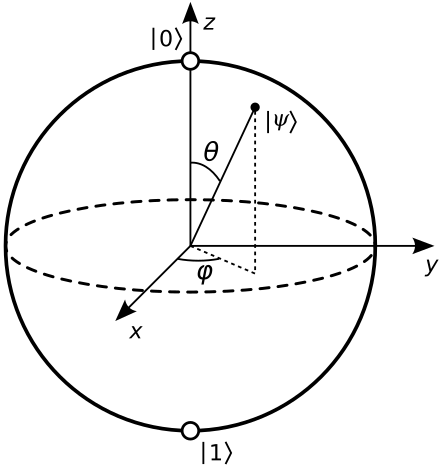
\includegraphics[width=0.6\textwidth]{02_Fundamentals_of_Quantum_Computing/bloch_sphere}
    \caption{The Bloch sphere representation of a single qubit state $|\psi\rangle = \cos(\theta/2)|0\rangle + e^{i\phi}\sin(\theta/2)|1\rangle$. The north pole represents $|0\rangle$, the south pole $|1\rangle$.}
    \label{fig:bloch_sphere}
\end{figure}

\subsubsection*{Physical Implementations}
Realizing qubits physically presents diverse approaches, each with unique advantages and challenges:
\begin{itemize}
    \item \textbf{Superconducting Circuits:} Utilize circuits with Josephson junctions cooled to milli-Kelvin temperatures. These allow for fast gate operations (nanoseconds) and are a leading technology, but require significant cryogenic infrastructure and are sensitive to noise.
    \item \textbf{Trapped Ions:} Individual charged atoms confined by electromagnetic fields. They boast very long coherence times (seconds to minutes) and high gate fidelities, but gate operations are typically slower (microseconds).
    \item \textbf{Photonic Qubits:} Employ quantum states of light (e.g., polarization or path encoding). Photons are naturally robust against decoherence and ideal for communication (Quantum Key Distribution), but building universal quantum gates for computation is challenging.
    \item \textbf{Other Platforms:} Include neutral atoms, quantum dots, topological qubits, and NV-centers in diamond, each representing active areas of research.
\end{itemize}
A major engineering challenge common to all platforms is maintaining quantum coherence—preserving the delicate superposition and entanglement against environmental noise (e.g., thermal fluctuations, stray electromagnetic fields) which causes decoherence (loss of quantum information). This necessitates sophisticated control systems, shielding, and often, operation at extremely low temperatures or high vacuum.

\subsection{Entanglement}\label{subsec:entanglement}
Quantum entanglement is a unique quantum correlation where two or more qubits become linked in such a way that they share the same fate, regardless of the distance separating them. Their states are described by a single, combined quantum state, not independent individual states. For example, if two qubits are entangled in the Bell state:
\begin{equation*}
    |\Phi^+\rangle = \frac{1}{\sqrt{2}}(|00\rangle + |11\rangle)
\end{equation*}
measuring the first qubit to be $|0\rangle$ instantly forces the second qubit to be $|0\rangle$, and measuring the first as $|1\rangle$ forces the second to be $|1\rangle$, even if they are light-years apart. This correlation, famously dubbed "spooky action at a distance" by Einstein, cannot be explained by classical physics (e.g., hidden variables) and is experimentally verified. While entanglement does not allow faster-than-light communication (information transfer still requires classical communication), it is a crucial resource enabling quantum algorithms (like Shor's), quantum teleportation, and certain quantum cryptographic protocols.

\section{Quantum Gates and Circuits}\label{sec:quantum_gates}

Quantum computations are performed by applying sequences of \textbf{quantum gates} to qubits. These gates are analogous to classical logic gates but operate on quantum states. Mathematically, single-qubit gates are represented by $2 \times 2$ unitary matrices ($U^\dagger U = I$), and multi-qubit gates by larger unitary matrices, ensuring that the evolution of quantum states is reversible and preserves probabilities. Below are examples of important quantum gates:

\subsection*{Pauli-X (NOT) Gate}
The Pauli-X gate acts as a quantum bit-flip, analogous to the classical NOT gate. It transforms $|0\rangle$ to $|1\rangle$ and $|1\rangle$ to $|0\rangle$. For a general qubit $|\psi\rangle = \alpha|0\rangle + \beta|1\rangle$:
\begin{equation*}
    X|\psi\rangle = X(\alpha|0\rangle + \beta|1\rangle) = \alpha|1\rangle + \beta|0\rangle
\end{equation*}
Matrix form:
\begin{equation*}
    X = \begin{pmatrix} 0 & 1 \\ 1 & 0 \end{pmatrix}
\end{equation*}

\subsection*{Pauli-Y Gate}
The Pauli-Y gate performs a bit-flip combined with phase changes.
\begin{equation*}
    Y|\psi\rangle = Y(\alpha|0\rangle + \beta|1\rangle) = \alpha(i|1\rangle) + \beta(-i|0\rangle) = -i\beta|0\rangle + i\alpha|1\rangle
\end{equation*}
Matrix form:
\begin{equation*}
    Y = \begin{pmatrix} 0 & -i \\ i & 0 \end{pmatrix}
\end{equation*}

\subsection*{Pauli-Z Gate}
The Pauli-Z gate acts as a phase-flip, leaving $|0\rangle$ unchanged and mapping $|1\rangle$ to $-|1\rangle$.
\begin{equation*}
    Z|\psi\rangle = Z(\alpha|0\rangle + \beta|1\rangle) = \alpha|0\rangle - \beta|1\rangle
\end{equation*}
Matrix form:
\begin{equation*}
    Z = \begin{pmatrix} 1 & 0 \\ 0 & -1 \end{pmatrix}
\end{equation*}

\subsection*{Hadamard (H) Gate}
The Hadamard gate is crucial for creating superposition. It transforms $|0\rangle$ into an equal superposition of $|0\rangle$ and $|1\rangle$, and $|1\rangle$ into an equal superposition with a phase difference.
\begin{equation*}
    H|0\rangle = \frac{|0\rangle + |1\rangle}{\sqrt{2}}, \quad H|1\rangle = \frac{|0\rangle - |1\rangle}{\sqrt{2}}
\end{equation*}
Applying H twice returns the original state ($H^2 = I$).
Matrix form:
\begin{equation*}
    H = \frac{1}{\sqrt{2}}\begin{pmatrix} 1 & 1 \\ 1 & -1 \end{pmatrix}
\end{equation*}

\subsection*{Phase (S or $\sqrt{Z}$) Gate}
The S gate introduces a relative phase shift of $\pi/2$ (or $i$) between the $|0\rangle$ and $|1\rangle$ components. It is sometimes called the $\sqrt{Z}$ gate as $S^2 = Z$.
\begin{equation*}
    S|\psi\rangle = S(\alpha|0\rangle + \beta|1\rangle) = \alpha|0\rangle + i\beta|1\rangle
\end{equation*}
Matrix form:
\begin{equation*}
    S = \begin{pmatrix} 1 & 0 \\ 0 & i \end{pmatrix}
\end{equation*}

\subsection*{T (or $\pi/8$) Gate}
The T gate introduces a relative phase shift of $\pi/4$. It is important because H, S, and CNOT gates alone are not sufficient for universal quantum computation; adding the T gate completes a common universal set.
\begin{equation*}
    T|\psi\rangle = T(\alpha|0\rangle + \beta|1\rangle) = \alpha|0\rangle + e^{i\pi/4}\beta|1\rangle
\end{equation*}
Matrix form:
\begin{equation*}
    T = \begin{pmatrix} 1 & 0 \\ 0 & e^{i\pi/4} \end{pmatrix} = \begin{pmatrix} 1 & 0 \\ 0 & \frac{1+i}{\sqrt{2}} \end{pmatrix}
\end{equation*}

\subsection*{CNOT (Controlled-NOT) Gate}
The CNOT gate is a fundamental two-qubit gate. It flips the state of the second qubit (target) if and only if the first qubit (control) is in the state $|1\rangle$.
\begin{align*}
    \text{CNOT}|00\rangle &= |00\rangle \\
    \text{CNOT}|01\rangle &= |01\rangle \\
    \text{CNOT}|10\rangle &= |11\rangle \\
    \text{CNOT}|11\rangle &= |10\rangle
\end{align*}
Matrix form (acting on basis states $|00\rangle, |01\rangle, |10\rangle, |11\rangle$):
\begin{equation*}
    \text{CNOT} = \begin{pmatrix} 1 & 0 & 0 & 0 \\ 0 & 1 & 0 & 0 \\ 0 & 0 & 0 & 1 \\ 0 & 0 & 1 & 0 \end{pmatrix}
\end{equation*}
The CNOT gate is essential for creating entanglement and is a key component in many quantum algorithms and error correction codes.

\subsection*{Toffoli (CCNOT) Gate}
The Toffoli gate is a three-qubit gate, acting as a controlled-controlled-NOT. It flips the third qubit if and only if the first two control qubits are both in the state $|1\rangle$.
\begin{equation*}
    \text{CCNOT}|abc\rangle = |ab(c\oplus(a\cdot b))\rangle
\end{equation*}
where $\oplus$ is addition modulo 2.
Matrix form (acting on basis states $|000\rangle$ through $|111\rangle$):
\begin{equation*}
    \text{CCNOT} = \begin{pmatrix}
    1&0&0&0&0&0&0&0 \\
    0&1&0&0&0&0&0&0 \\
    0&0&1&0&0&0&0&0 \\
    0&0&0&1&0&0&0&0 \\
    0&0&0&0&1&0&0&0 \\
    0&0&0&0&0&1&0&0 \\
    0&0&0&0&0&0&0&1 \\ % Flips |110> to |111>
    0&0&0&0&0&0&1&0  % Flips |111> to |110>
    \end{pmatrix}
\end{equation*}
The Toffoli gate is universal for classical reversible computation. Together with the Hadamard gate (or other suitable single-qubit rotations), it forms a universal set for quantum computation, meaning any quantum computation can be decomposed into a sequence of these gates.

\subsection*{Bell States Creation}
Applying a Hadamard gate to the first qubit (initially $|0\rangle$) followed by a CNOT gate controlled by the first qubit acting on the second (initially $|0\rangle$) creates the Bell state $|\Phi^+\rangle$:
\begin{enumerate}
    \item Start with $|00\rangle$.
    \item Apply H to the first qubit: $H|0\rangle \otimes |0\rangle = \frac{1}{\sqrt{2}}(|0\rangle + |1\rangle) \otimes |0\rangle = \frac{1}{\sqrt{2}}(|00\rangle + |10\rangle)$.
    \item Apply CNOT (control=1st, target=2nd): $\text{CNOT} \left( \frac{1}{\sqrt{2}}(|00\rangle + |10\rangle) \right) = \frac{1}{\sqrt{2}}(|00\rangle + |11\rangle) = |\Phi^+\rangle$.
\end{enumerate}
This maximally entangled state demonstrates how quantum gates can generate non-classical correlations essential for quantum algorithms.

\section{Quantum Algorithms}\label{sec:quantum_algorithms}

Quantum algorithms leverage the principles of superposition, entanglement, and quantum interference to perform computations in ways that can dramatically outperform classical algorithms for specific problems. This section introduces three cornerstone quantum algorithms: the Quantum Fourier Transform (QFT), Quantum Phase Estimation (QPE), and Amplitude Amplification (which generalizes Grover's search algorithm), highlighting their mechanisms, interdependencies, and cryptographic relevance.

\subsection{Quantum Fourier Transform (QFT)}\label{subsec:qft}
The Quantum Fourier Transform (QFT) is the quantum analogue of the classical Discrete Fourier Transform (DFT). It maps a quantum state represented in the computational basis to its representation in the Fourier basis. Its primary strength lies in efficiently finding periodicities in quantum states.

When applied to a computational basis state $|j\rangle$ (where $j$ is an integer represented by $n$ qubits), the QFT generates a superposition state:
\begin{equation}\label{eq:qft}
    \text{QFT}|j\rangle = \frac{1}{\sqrt{N}} \sum_{k=0}^{N-1} e^{2\pi i jk/N} |k\rangle
\end{equation}
where $N=2^n$ is the dimension of the state space. While a classical Fast Fourier Transform (FFT) takes $\mathcal{O}(N\log N)$ operations, the QFT circuit can be implemented using only $\mathcal{O}(n^2) = \mathcal{O}((\log N)^2)$ quantum gates (Hadamard and controlled phase rotations $R_m$), offering an exponential speedup in terms of $n$.

\begin{figure}[h]
    \centering
    % Ensure the image path is correct relative to the main.tex file
    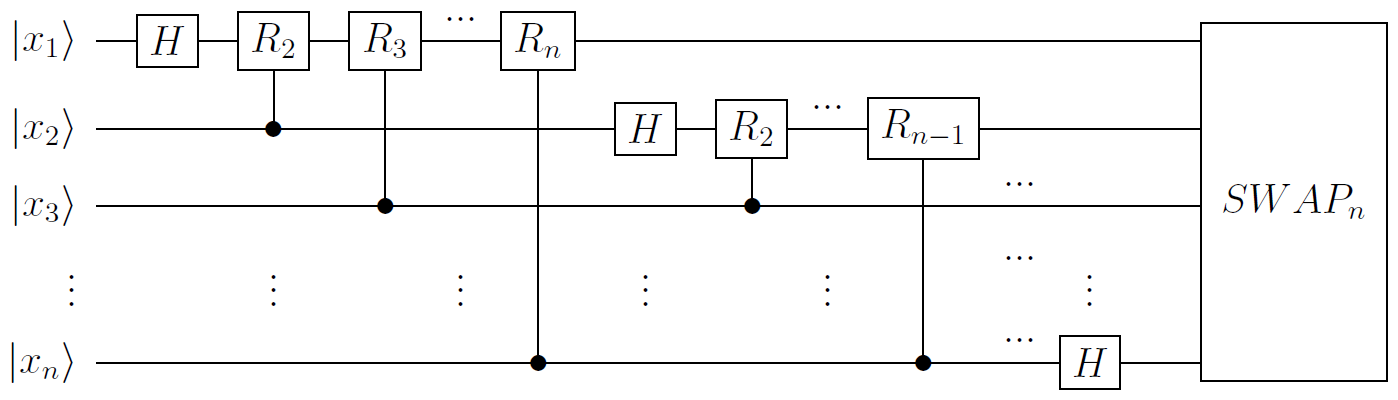
\includegraphics[width=0.8\textwidth]{02_Fundamentals_of_Quantum_Computing/qft_circuit}
    \caption{Quantum circuit implementing the QFT using layered Hadamard gates (H) and controlled phase rotations ($R_m$). Qubit ordering typically assumes $|x_1\rangle$ is the most significant qubit and $|x_n\rangle$ the least significant.}
    \label{fig:qft_circuit}
\end{figure}

The phase rotation gates $R_m$ are defined by:
\begin{equation}\label{eq:phase_gate}
    R_m = \begin{pmatrix} 1 & 0 \\ 0 & e^{2\pi i /2^m} \end{pmatrix}
\end{equation}
These gates apply progressively smaller phase shifts.

\textbf{Cryptographic Relevance:} The QFT's ability to efficiently find periods is the core component enabling \textbf{Shor's algorithm} to factor large integers and compute discrete logarithms exponentially faster than the best known classical algorithms. Shor's algorithm uses the QFT to find the period of the modular exponentiation function $f(x) = a^x \bmod N$, which then allows efficient calculation of the factors of $N$ or the discrete logarithm.

\subsection{Quantum Phase Estimation (QPE)}\label{subsec:qpe}
Quantum Phase Estimation is a fundamental quantum algorithm used to determine the eigenvalue (specifically, the phase) of an eigenvector of a unitary operator. Given a unitary operator $U$ and one of its eigenstates $|\psi\rangle$ such that $U|\psi\rangle = e^{2\pi i\theta}|\psi\rangle$, QPE efficiently estimates the phase $\theta \in [0, 1)$.

The algorithm uses two registers: the first (measurement register) with $m$ qubits initialized to $|0\rangle^{\otimes m}$, and the second (target register) initialized to the eigenstate $|\psi\rangle$.
Key steps:
\begin{enumerate}
    \item Apply Hadamard gates to the first register: $\frac{1}{\sqrt{2^m}}\sum_{k=0}^{2^m-1}|k\rangle \otimes |\psi\rangle$.
    \item Apply controlled-$U^{2^j}$ operations (controlled by the $j$-th qubit of the first register) to the second register. This encodes the phase $\theta$ into the first register's state: $\frac{1}{\sqrt{2^m}} \sum_{k=0}^{2^m-1} e^{2\pi i\theta k} |k\rangle \otimes |\psi\rangle$.
    \item Apply the inverse Quantum Fourier Transform (QFT$^{-1}$) to the first register.
    \item Measure the first register. The measurement outcome provides an $m$-bit approximation of $\theta$.
\end{enumerate}
The precision of the estimate scales as $2^{-m}$.

\begin{figure}[h]
\centering
 % Ensure the image path is correct relative to the main.tex file
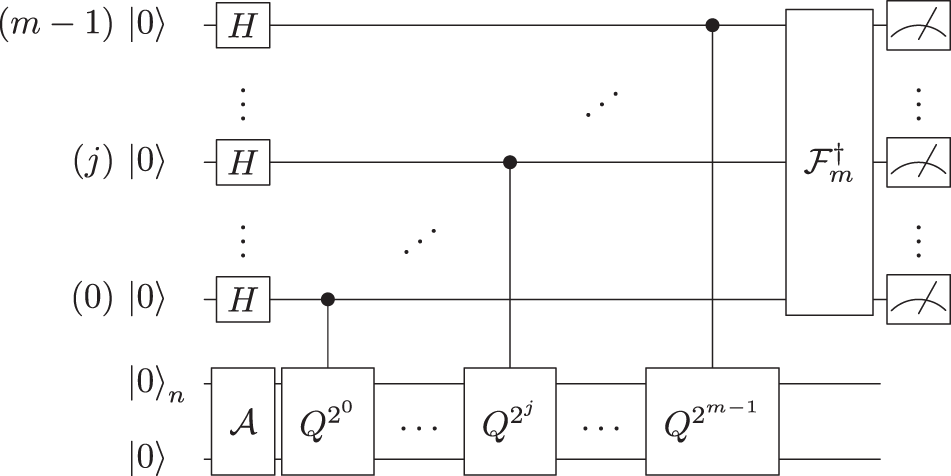
\includegraphics[width=0.8\textwidth]{02_Fundamentals_of_Quantum_Computing/qpe_circuit}
\caption{Quantum circuit for Phase Estimation. The top $m$ qubits form the measurement register, the bottom $n$ qubits hold the eigenstate $|\psi\rangle$. QFT$^{-1}$ is the inverse Quantum Fourier Transform.}
\label{fig:qpe_circuit}
\end{figure}

\textbf{Cryptographic Relevance:} QPE is the subroutine within \textbf{Shor's algorithm} that actually extracts the period information. The modular exponentiation operation can be implemented as a unitary operator $U$, and QPE is used to estimate the phase related to its eigenvalues, which in turn reveals the period needed for factoring or solving the discrete logarithm problem.

\subsection{Amplitude Amplification (Grover's Algorithm)}\label{subsec:amplitude_amp}
Amplitude Amplification is a general quantum technique for boosting the probability of measuring a desired ('good' or 'marked') state from a superposition. \textbf{Grover's search algorithm} is the most famous application, designed to find a specific item in an unsorted database (or search space) of size $N$.

Classically, finding the marked item requires, on average, $N/2$ queries (and $N$ in the worst case). Grover's algorithm achieves this with only $\mathcal{O}(\sqrt{N})$ quantum queries, providing a quadratic speedup. It doesn't offer the exponential speedup of Shor's algorithm but is applicable to a wider range of problems.

The algorithm works by iteratively rotating the quantum state vector towards the 'good' state(s). Suppose an initial state $|\psi\rangle$ is a superposition of 'good' states $|G\rangle$ and 'bad' states $|B\rangle$: $|\psi\rangle = \sin\theta|G\rangle + \cos\theta|B\rangle$, where the initial probability of finding a good state is $p = \sin^2\theta \approx M/N$ (if there are $M$ good states out of $N$). The core Grover iteration involves two reflections:
\begin{enumerate}
    \item Reflection about the subspace orthogonal to the good states ($U_G = I - 2|G\rangle\langle G|$).
    \item Reflection about the initial state $|\psi\rangle$ ($U_\psi = I - 2|\psi\rangle\langle\psi|$).
\end{enumerate}
The combined operation $Q = -U_\psi U_G$ rotates the state vector by $2\theta$ towards $|G\rangle$. After approximately $\frac{\pi}{4\theta} \approx \frac{\pi}{4}\sqrt{N/M}$ iterations, the amplitude of the good state(s) is maximized, allowing measurement with high probability.

% Commenting out missing image placeholder
%\begin{figure}[h]
%    \centering
%    \includegraphics[width=0.7\textwidth]{amplitude_amplification}
%    \caption{Geometric visualization of amplitude amplification as a rotation in the plane spanned by the good state $|G\rangle$ and the orthogonal bad state $|B\rangle$.}
%    \label{fig:amplitude_amp}
%\end{figure}

\textbf{Cryptographic Relevance:} Grover's algorithm directly threatens cryptographic primitives that rely on computational difficulty of search:
\begin{itemize}
    \item \textbf{Symmetric Key Cryptography:} Finding the correct $n$-bit key for a cipher like AES can be viewed as searching a space of $N=2^n$ possible keys. Grover reduces the effective search time from $\mathcal{O}(2^n)$ to $\mathcal{O}(\sqrt{2^n}) = \mathcal{O}(2^{n/2})$. This effectively halves the bit security of symmetric keys against quantum adversaries (e.g., AES-128 becomes equivalent to 64-bit security, AES-256 to 128-bit security).
    \item \textbf{Hash Functions:} Finding a pre-image (given $h$, find $x$ such that $H(x)=h$) or a second pre-image for an $n$-bit hash function is also a search problem over a large space. Grover reduces the effective complexity from $\mathcal{O}(2^n)$ to $\mathcal{O}(2^{n/2})$. Collision finding complexity is also reduced, typically to around $\mathcal{O}(2^{n/3})$ or $\mathcal{O}(2^{n/2})$ depending on the specific quantum collision-finding algorithm.
\end{itemize}
The standard mitigation against Grover's algorithm is to double the key lengths (for symmetric ciphers) or output lengths (for hash functions) to maintain the desired classical security level.

\subsection{Algorithm Interconnections and Cryptographic Impact Summary}\label{subsec:algo_connections}
The fundamental algorithms QFT, QPE, and Amplitude Amplification form an interconnected toolkit with profound cryptographic implications:
\begin{itemize}
    \item \textbf{QFT and QPE} are the core components of \textbf{Shor's algorithm}. They provide an *exponential* speedup for problems like integer factorization and discrete logarithms (both standard and elliptic curve variants). This completely breaks the security foundations of current public-key cryptosystems like RSA, Diffie-Hellman, and ECC.
    \item \textbf{Amplitude Amplification (Grover's algorithm)} provides a *quadratic* speedup for unstructured search problems. This weakens, but does not completely break, symmetric-key ciphers (like AES) and hash functions (like SHA-2, SHA-3) by effectively halving their bit security against brute-force style attacks.
\end{itemize}
Understanding these algorithms and their impact is crucial for appreciating the need for post-quantum cryptography, as discussed in later chapters.

% Commenting out missing image placeholder
%\begin{figure}[h]
%    \centering
%    \includegraphics[width=0.8\textwidth]{algorithm_relationships}
%    \caption{Relationships between fundamental quantum algorithms and their cryptographic impact}
%    \label{fig:algo_relationships}
%\end{figure}

\section{The NISQ Era and Beyond}\label{sec:nisq_era}
While the theoretical power of quantum algorithms like Shor's is clear, their practical implementation faces immense hurdles. We currently operate in the \textbf{Noisy Intermediate-Scale Quantum (NISQ)} era, a term coined by John Preskill \parencite{preskill2018quantum}. NISQ devices are characterized by:
\begin{itemize}
    \item \textbf{Intermediate Scale:} Possessing roughly 50 to a few thousand qubits. This is insufficient for running Shor's algorithm against cryptographically relevant key sizes.
    \item \textbf{Noisy Qubits:} Qubits and quantum gates are imperfect and susceptible to errors from decoherence and imperfect control. Error rates are too high for complex computations without error correction.
    \item \textbf{Lack of Fault Tolerance:} NISQ devices do not employ full-scale quantum error correction (QEC).
\end{itemize}

\textbf{Quantum Error Correction (QEC)} is theoretically capable of overcoming noise by encoding information redundantly across many physical qubits to create a more stable "logical qubit". However, QEC codes (like the surface code) have extremely high overheads. Current estimates suggest that factoring a 2048-bit RSA number using Shor's algorithm might require millions of high-quality physical qubits to encode the necessary thousands of logical qubits \parencite{gidney2021factor}. This resource requirement far exceeds the capabilities of current NISQ hardware.

This discrepancy creates the \textbf{"Quantum Advantage Gap"}: we possess algorithms known to break current cryptography, but lack the hardware technology to execute them at scale. Bridging this gap is a central goal of quantum computing research, focusing on:
\begin{itemize}
    \item Building more stable, higher-fidelity physical qubits with longer coherence times.
    \item Developing more efficient QEC codes and fault-tolerant architectures.
    \item Improving quantum compilation techniques to minimize resource requirements.
    \item Designing potentially useful algorithms that might run effectively on NISQ devices or require fewer resources than initially thought.
    \item Exploring hybrid quantum-classical approaches that leverage the strengths of both paradigms.
\end{itemize}
Although the timeline for fault-tolerant quantum computing capable of breaking RSA-2048 remains uncertain (with estimates ranging widely), the potential impact necessitates proactive migration to quantum-resistant cryptography.